\chapter{Financial risk modeling}\label{ch:4}

\begin{remark}{Outline}
\todo{fix outline}
In this chapter, we present the well-known family of \textit{random forests}
methods. In Section~\ref{sec:4:bias-variance}, we first describe the bias-variance
decomposition of the prediction error and then present, in
Section~\ref{sec:4:ensemble}, how aggregating randomized models through
ensembles reduces the prediction error by decreasing the variance term in this
decomposition. In Section~\ref{sec:4:random-forests}, we revisit random forests
and its variants and study how randomness introduced into the decision trees
reduces prediction errors by decorrelating the decision
trees in the ensemble. Properties and features of random forests are then outlined
in Section~\ref{sec:4:features} while their consistency
is finally explored in Section~\ref{sec:4:consistency}.
\end{remark}

\section{Credit card fraud detection}

	Every year billions of Euros are lost worldwide due to credit card fraud. Thus, leading financial 
	institutions to continuously improve their fraud detection systems. In recent years, several 
	studies have proposed the use of machine learning and data mining techniques to address this 
	problem. However, most studies used some sort of misclassification measure to evaluate the 
	different solutions, and by doing so, missed to take into account the actual financial costs 
	associated with the fraud detection process. Moreover, when constructing a credit card fraud 
	detection model, it is very important how to 	preprocess the transactional data. This is usually 
	done by aggregating the transactions in order 	to observe the spending behavioral patterns of 
	the customers. In this work, we expand the transaction aggregation strategy, and also propose a 
	creating new set 	of features based in analyzing the periodic behavior of the time of a 
	transaction using the von 	Mises distribution. Then, using a real credit card fraud dataset 
	provided by a large European card processing company, we compare state-of-the-art credit card 
	fraud detection models, and evaluate how the 	different sets of features have an impact on the 
	results. By including the proposed periodic features into the methods, 	the results show an 
	average increase in the savings of 12.55\%
	\todo{erase percentage of savings}
	
\subsection{Introduction}

  The use of credit and debit cards has increased significantly   in the last years, unfortunately 
	so has the fraud. Because of it, billions of Euros are lost every year. According to 
	the European Central Bank \citep{EuropeanCentralBank2013}, during 2012 the total level of fraud 
	reached 1.33 billion Euros in the Single Euro Payments Area, which represents an increase of 
	14.8\% compared with 2011. Moreover, payments across non traditional channels (mobile, internet, 
	...) accounted for 60\% of the fraud, whereas it was 46\% in 2008. This open new challenges as 
	new fraud patterns emerge, and current fraud detection systems are not being successful in 
	preventing fraud. Furthermore, fraudsters constantly change their strategies to avoid being 
	detected, something that makes traditional fraud detection tools such as expert rules inadequate.
  
  The use of machine learning in fraud detection has been an interesting topic in recent years. 
  Several detection systems based on machine learning techniques has been successfully used 
	for this problem \citep{Bhattacharyya2011}. When constructing a credit card fraud detection 
model, 
	there are several problems that have an important impact during the training phase: Skewness of 	
	the data , cost-sensitivity of the application, short time response of the system, dimensionality 
	of the search space and how to preprocess the features
	\citep{Bolton2002,Gadi2008,Whitrow2008,DalPozzolo2014}.	In this paper, we are interested to 
	address the cost-sensitivity and the features preprocessing 	issues. 
	
	A credit card fraud detection is by definition a cost-sensitive problem, in the sense that the 
	cost 	due a false positive is different than the cost of a false negative. ie. When predicting a 	
	transaction 	as fraudulent when in fact it is not a fraud there is an administrative cost that 	
	is incurred by 	the financial institution, on the other hand, when failing to detect a fraud, the 
	amount of that 	transaction is loss \citep{Hand2007a}. Moreover, it is not enough  to assume a 	
	constant cost 	difference between false positives and false negatives, as the amount of the 	
	transactions vary 	quite significantly, therefore, its financial impact is not constant but 	
	depended on each 	transaction.	In \citep{CorreaBahnsen2013}, we propose a new cost-based measure 
	to evaluate 	credit card fraud detection models, taking into account the different financial 	
	costs incurred by 	the fraud detection process.
	
	When constructing a credit card fraud detection model, it is very important to use those features 
	that will help the algorithm make the best decision. Typical models only use the raw 
	transactional features, such as the time, amount, place of the transaction. However, this 
approach 
	do not take into account the spending behavior of the customer, which is expected to help 
	discover fraud patterns. A standard way to include these behavioral spending patters was proposed 
	in \citep{Whitrow2008}, they propose a transaction aggregation strategy in order to take into 
	account a customer spending behavior. The derivation of the aggregated features consists in 
	grouping the transactions made during the last given number of hours, first by card or account 
	number, then by transaction type, merchant group, country or other, followed by calculating
	the number of transactions or the total amount spent on those transactions.
	
	In this paper, we propose an expanded version of the transaction aggregation strategy, by 
	incorporate a combination criteria when grouping the transaction. ie. instead of aggregating only 
	by card holder and transaction type, we combine it with country or merchant group, this allow to 
	have a much richer feature space. Moreover, there is still some information that is not 
	completely captured by the aggregated features. In particular we are interesting in analyzing the 
	time of the transaction. The logic behind this, is that a customer is expected to make 
	transactions at similar hours. We propose a new method for creating features  based in the 
	periodic behavior of a transaction time, using the von Mises distribution. In particular, the new 
	features estimate if the time of a new transaction is within the confidence interval of the 
	previous transaction times. 
	
	Furthermore, using a real credit card fraud dataset provided by a large European card processing 
	company, we compare the different sets of 	features (raw, aggregated and periodic), using 
	different cost-insensitive and 	cost-sensitive machine learning algorithms. In particular, we 
	used the cost-insensitive algorithms logistic regression, decision trees and random forest 
	\citep{Hastie2009}, and the 	cost-sensitive methods 	cost-proportionate sampling 
	\citep{Elkan2001,Zadrozny2003}, Bayes minimum 	risk 	\citep{CorreaBahnsen2013}, cost-sensitive 
	logistic regression \citep{CorreaBahnsen2014b} 	and 	cost-sensitive decision trees 
	\citep{CorreaBahnsen2015}. The results show an average increase in the savings of 12.55\% by 
using 
	the proposed periodic features. Additionally, the outcome of this paper is being currently used 
	to implement a state-of-the-art fraud detection 	system, that will  help to combat 	fraud once 
	the implementation stage is finished. 

	The remainder of the paper is organized as follows. In Section 2, we explain the 
	background on credit card fraud detection, including our recently proposed example-dependent 
	cost-sensitive evaluation measures. Then in Section 3, we discuss current 	approaches to create 
	the features used in fraud detection models, moreover, we present our 	proposed methodology to 
	create periodic based features. Afterwards, the experimental setup and 	the results are given in 
	Section 4. Finally, conclusions of the paper are presented in 	\mbox{Section 5}. 

\subsection{Credit card fraud detection evaluation}
\label{sec:4:frad:eval}

	A credit card fraud detection algorithm, consist in identifying those transactions with a 
	high probability of being fraud, based on historical fraud patterns. 
  The use of machine learning in fraud detection has been an interesting topic in recent years. 
	However, due to the confidentiality of financial information and non availability of public 
	databases, few researches have had the opportunity to work on developing methods specific 
	to credit card fraud detection \citep{Bolton2002,DalPozzolo2014}.
	
	Nevertheless, different detection systems that are based on machine learning 
	techniques have been successfully used for this problem, in particular: neural 
	networks~\citep{Maes2002}, Bayesian learning \citep{Maes2002}, artificial immune systems 
	\citep{Gadi2008}, association rules \citep{Sanchez2009}, hybrid models \citep{Krivko2010}, 
	support vector machines~\citep{Bhattacharyya2011}, peer group  analysis \citep{Weston2008}, 
	random forest~\citep{CorreaBahnsen2013} and online learning \citep{DalPozzolo2014}.

  Most of these studies compare they proposed algorithm with a benchmark algorithm and then make 
	the comparison using a standard binary classification measure, such as misclassification error, 
	receiver operating characteristic ($ROC$), Kolmogorov-Smirnov ($KS$) or \mbox{$F_1Score$} 
	statistics \citep{Bolton2002,Hand2007a,DalPozzolo2014}. Most of these measures are extracted by 
	using a confusion matrix as shown in \tablename{ \ref{confusion}}. Where the prediction of the 
	algorithm $c_i$ is a function of  the $k$ features of example $i$, \mbox{$\mathbf{X}_i=[x_i^1, 
	x_i^2,...,x_i^k]$} and $y_i$ is the true class of the example $i$.

	\begin{table}[b]
		\caption{Classification confusion matrix}
		\centering
    \begin{tabular}{c|c|c}
      \multicolumn{3}{c}{}\\
			\multicolumn{1}{c|}{}  & Actual Positive& Actual Negative \\
			\multicolumn{1}{c|}{} & $y=1$& $y=0$ \\
			\hline
			Predicted Positive 		& \multirow{ 2}{*}{True Positive ($TP$)} & \multirow{ 
			2}{*}{False Positive ($FP$)} \\
			$c=1$ & &\\
			\hline
			Predicted Negative  	& \multirow{ 2}{*}{False Negative ($FN$)} & \multirow{ 
			2}{*}{True Positive ($TN$)} \\
			$c=0$ & &\\
		\end{tabular}
		\label{confusion}
  \end{table}  

	From this table several statistics are extracted. In particular:
	\begin{itemize}
		\item Accuracy = $\frac{TP+TN}{TP+TN+FP+FN}$
		\item Recall = $\frac{TP}{TP+FN}$
		\item Precision = $\frac{TP}{TP+FP}$
		\item $F_1Score = 2\frac{Precision \cdot Recall}{Precision + Recall}$
	\end{itemize}

	However, these measures may not be the most appropriate evaluation criteria when  evaluating a 
	fraud detection models, because they tacitly assume that misclassification errors carry the same 
	cost, similarly with the correct classified examples. This assumption does not hold in many 
	real-world applications such as fraud detection, since  when wrongly predicting a fraudulent 
	transaction as legitimate carries a significantly different financial cost than the inverse case.
	Furthermore, the accuracy measure also assumes that the class distribution among examples is 
	constant and balanced \citep{Provost1998}, and typically the distributions of a fraud detection 
	data set are skewed, with a percentage of frauds ranging from 0.005\% to 0.5\% 
	\citep{Gadi2008,Bhattacharyya2011}.

	In order to take into account the different costs of fraud detection during the evaluation of an 
	algorithm, we used the cost matrix as defined in \citep{Elkan2001}. In \tablename{  
	\ref{tab:table_costmat}}, the cost matrix is presented, where the cost associated with two types 
	of correct classification, namely, true positives $C_{TP_i}$, and true negatives $C_{TN_i}$; and 
	the two types of misclassification errors, namely, false positives $C_{FP_i}$, and false 
	negatives  $C_{FN_i}$, are presented.

	\begin{table}[b]
		\caption{Cost matrix \citep{Elkan2001}}
		\centering
		\begin{tabular}{c|c|c}
		\multicolumn{3}{c}{}\\
			\multicolumn{1}{c|}{}  & Actual Positive& Actual Negative \\
			\multicolumn{1}{c|}{} & $y_i=1$& $y_i=0$ \\
			\hline
			Predicted Positive 		& \multirow{ 2}{*}{$C_{TP_i}$} & \multirow{ 2}{*}{$C_{FP_i}$} 
			\\
			$c_i=1$ & &\\
			\hline
			Predicted Negative  	& \multirow{ 2}{*}{$C_{FN_i}$} & \multirow{ 
			2}{*}{$C_{TN_i}$} \\
			$c_i=0$ & &\\
			%\hline
		\end{tabular}
		\label{tab:table_costmat}
	\end{table}  

	Hand et al. \citep{Hand2007a} proposed a cost matrix, where in the case of false positive the 
	associated 	cost is the administrative cost $C_{FP_i}=C_a$ related to analyzing the transaction 
	and contacting 	the card holder. This cost is the same assigned to a true positive 
	$C_{TP_i}=C_a$, because in 	this case, 	the card holder will have to be contacted. However, in 
	the case of a false negative, in which a 	fraud is 	not detected, the cost is defined to be a 
	hundred times $C_{FN_i}=100C_a$. This same approach was also used in \citep{Gadi2008}.

	Nevertheless, in 	practice, losses due to a specific fraud 	range from few to 
	thousands of Euros, which means that 	assuming constant cost for false 	negatives is 	
	unrealistic. In order to address this limitation, in 	\citep{CorreaBahnsen2013}, we 	proposed a 
	cost matrix that take into account the actual 	example-dependent financial costs. Our 	cost 
	matrix define the cost of a false negative to be the 	amount $C_{FN_i}=Amt_i$ of the 	transaction 
	$i$. This cost matrix is a better representation of the 	actual costs, since when a 	fraud is 
	not detected, the losses of that particular fraud correspond 	to the stolen amount.
	The costs are summarized in \tablename{ \ref{tab:table_costmat_fraud}}.

	Afterwards, using the example-dependent cost matrix a cost measure is calculated taking into 
	account the actual costs \mbox{$\mathbf{C}_i=[C_{TP_i},C_{FP_i},C_{FN_i},C_{TN_i}]$} of each 
	example $i$. Let $\mathcal{S}$ be a set of $N$ examples $i$, $N=\vert \mathcal{S} \vert$, where 
	each example is represented by the augmented feature vector \mbox{$\mathbf{X}_i'=[\mathbf{X}_i, 
	\mathbf{C}_i]$}, and labelled using the class label $y_i \in \{0,1\}$. A classifier $f$ which 
	generates the predicted label $c_i$ for each example $i$, is trained using the set $\mathcal{S}$. 
	Then the cost of using $f$ on $\mathcal{S}$ is \mbox{calculated by}
  \begin{align}
    Cost(f(\mathcal{S})) &= \sum_{i=1}^{N} \bigg( y_i(c_i C_{TP_i} + (1-c_i)C_{FN_i})  \nonumber\\ 
    & +(1-y_i)(c_i C_{FP_i} + (1-c_i)C_{TN_i}) \bigg). \nonumber \\
	  &=  \sum_{i=1}^{N} y_i(1-c_i)Amt_i + c_iC_a
  \end{align} \label{eq:cost}

	\begin{table}[t]
		\caption{Credit card fraud cost matrix \citep{CorreaBahnsen2013}}
		\centering
		\begin{tabular}{c | c | c }
		\multicolumn{3}{c}{}\\
			\multicolumn{1}{c|}{}  & Actual Positive& Actual Negative \\
			\multicolumn{1}{c|}{} & $y_i=1$& $y_i=0$ \\
			\hline
			Predicted Positive 		& \multirow{ 2}{*}{$C_{TP_i}=C_a$} & \multirow{ 2}{*}{$C_{FP_i}=C_a$} 
			\\
			$c_i=1$ & &\\
			\hline
			Predicted Negative  	& \multirow{ 2}{*}{$C_{FN_i}=Amt_i$} & \multirow{ 
			2}{*}{$C_{TN_i}=0$} \\
			$c_i=0$ & &\\
			%\hline
		\end{tabular}
		\label{tab:table_costmat_fraud}
	\end{table}
	  
	However, as noted in \citep{Whitrow2008}, the total cost may not be easy to interpret. So they 
	propose a normalized cost measure, by dividing the total cost by the theoretical maximum cost, 
	which is the cost of misclassifying every example.
  \begin{align}
    NCost(f(\mathcal{S})) &= \frac{\sum_{i=1}^{N} y_i(1-c_i)Amt_i + c_iC_a}
							{\vert \mathcal{S}_0 \vert C_a + \sum_{i=1}^{N}Amt_i\cdot \mathbf{1}_1(y_i)},
  \end{align} \label{eq:ncost}
  where, $\mathcal{S}=\{\mathbf{X}_i'|y_i=0,i \in 1..N\}$, and $\mathbf{1}_c(z)$ is an 
	indicator function that takes the value of one if $z \in c$ and zero if $z \notin c$ .

	We propose a similar approach in \citep{CorreaBahnsen2015}. By defining the savings of using an 
	algorithm as the cost of the algorithm versus the cost of using no algorithm at all. 
	To do that, we set the cost of using no algorithm as 
	\begin{equation}
		Cost_l(\mathcal{S}) = \min \{Cost(f_0(\mathcal{S})), Cost(f_1(\mathcal{S}))\},
	\end{equation}
	where $f_0$ refers to a classifier that predicts all the examples in $\mathcal{S}$ as belonging 
	to the class $c_0$, and similarly $f_1$ 	predicts all the examples in $\mathcal{S}$ as belonging 
	to the class $c_1$, the cost improvement 	can be expressed as the cost savings as compared with 
	$Cost_l(\mathcal{S})$. 
  \begin{equation}\label{eq:savings}
    Savings(f(\mathcal{S})) = \frac{ Costl(\mathcal{S}) - 
		Cost(f(\mathcal{S}))}{Cost_l(\mathcal{S})}.
  \end{equation} 

	For out analysis we decide to use the savings measure instead of the normalized cost, since in 
	the field of credit card fraud detection it is often see that companies do not use predictive 
	models, therefore, the savings measure makes more sense in that scenario.
	Moreover, as discussed in \citep{CorreaBahnsen2013}, it is not enough to evaluate a model using a 
	cost-sensitive measure, but it should also be trained to take into account the cost-sensitivity 
	of the problem. In the following Section we make a brief introduction to state-of-the-art 
	example-dependent cost-sensitive classification algorithms.

	
\subsection{Fraud detection feature engineering}
\label{sec:4:frad:features}

	When constructing a credit card fraud detection algorithm, the initial set of features (raw 
	features) include information regarding individual transactions. It is observed throughout the 
	literature, that regardless of the study the set of raw features is quite similar. This is 
	because the data produce during a credit card transaction must comply with international 
	accounting rules. In \tablename{ \ref{tab:raw_features}}, the typical credit card fraud detection 
	raw features are summarized.
	
	\begin{table}[!t]
   \caption{Summary of typical raw credit card fraud detection features}
   \label{tab:raw_features}
   \centering
   \begin{tabular}{l l}
   \hline
   \textbf{Attribute name} & \textbf{Description}\\
   \hline
		Transaction ID & Transaction identification number \\
   Time & Date and time of the transaction\\
   Account number & Identification number of the customer\\
   Card number & Identification of the credit card\\
   Transaction type & ie. Internet, ATM, POS, ...\\
	 Entry mode & ie. Chip and pin, magnetic stripe, ...\\
   Amount & Amount of the transaction in Euros\\
   Merchant code & Identification of the merchant type\\
   Merchant group & Merchant group identification\\
   Country & Country of trx\\
   Country 2 & Country of residence \\
   Type of card & ie. Visa debit, Mastercard, American Express...\\
   Gender & Gender of the card holder\\
   Age & Card holder age\\
   Bank & Issuer bank of the card\\
   Fraud & Indicator whenever or not a transaction was a fraud\\
   \hline
   \end{tabular}
   \end{table}
	
	\subsubsection{Capturing customer spending patterns}
	\label{sec:4:frad:features_agg}
	
	Several studies, used only the raw features for doing their analysis 
	\citep{Brause1999a,Minegishi2011,Panigrahi2009,Sanchez2009}. However, as noted in 
	\citep{Bolton2001}, a single transaction information is not sufficient to detect a fraudulent 
	transaction. Moreover, it is also impractical, as using only the raw features leaves behind 
	important information such as the consumer spending behavior, which is usually used by commercial 
	fraud detection systems.
	
	To deal with this, in \citep{Gadi2008}, a new set of features where proposed such that the 
	information of the last transaction made with the same credit card is also used to make a 
	prediction. The objective, is to be able to detect very dissimilar continues transactions within 
	a	customer purchases. The new set of features include: Time since the last transaction, previous 	
	amount of the transaction, previous country of the transaction.
	Nevertheless, these features does not take into account consumer behavior other than the last 
	transaction made by a client, this leads to having an incomplete profile of the customers.
	
	A more compressive way to take into account a customer spending behavior is to derive some 
	features using a transaction aggregation strategy. This methodology was initially proposed in 
	\citep{Whitrow2008}.  The derivation of the aggregation features consists in  grouping 
	the transactions made during the last given number of hours, first by card or account number, 
	then by transaction type, merchant group, country or other, followed by calculating the number 
	of transactions or the total amount spent on those 	transactions. This methodology has been used 
	by a number of studies 
	\citep{Bhattacharyya2011,Weston2008,Tasoulis2008,CorreaBahnsen2013,Sahin2013,CorreaBahnsen2014,
DalPozzolo2014}.
	
	When aggregating a customer transactions, there is a important question of how much to 
	accumulate, in the sense that the marginal value of new information may diminish as time passes.
	\citep{Whitrow2008}, discuss that aggregating 101 transactions is not likely to be
	more informative that aggregating 100. Indeed, when time passes information loss their value, in 
	the sense that a customer spending patterns are not expected to remain constant over the years.
	In particular, Whitrow et al., define a fix time frames to be 24, 60 and 168 hours.
	
	The process of aggregating features consists in for each transaction $i$ on the dataset 
	$\mathcal{S}$, select 	those transactions that were made in the previous $t_p$ hours,
	\begin{equation}\label{eq:agg_features1}
		TRX_{agg}(\mathcal{S},i, t_p) = \bigg\{x_l^{amt} \bigg\vert \left(x_l^{id}=x_i^{id}\right) 
		\wedge \left(hours(x_i^{time},x_l^{time}) < t_p\right) \bigg\}_{l=1}^N,
	\end{equation}
	where $N=\vert\mathcal{S}\vert$, $x_i^{time}$ is the time of transaction $i$,  $x_i^{amt}$ is the 
	amount of transaction $i$, $x_i^{id}$  the customer identification number of transaction $i$, 
	and $hours(z_1,z_2)$ is 	a function that calculate the number of hours between the dates $z_1$ 
	and $z_2$. Afterwards the feature number of transactions and amount of transactions in the last 
	$t_p$ hours are calculated as:
	\[
		x_i^{a1} = \vert TRX_{agg}(\mathcal{S},i, t_p) \vert \quad  \text{and} \quad x_i^{a2} = \sum 
	TRX_{agg}(\mathcal{S},i, t_p).
	\]
	
	Furthermore, we observed that this aggregation is not enough, in the sense that the combination 
	of 	the different features is not being taken into account. For example, it is not only 
	interesting 	to see the total transactions, but instead grouped by 	certain criteria, such as: 
	transactions 	made in the last $t_p$ hours, in the same country 	and of the same transaction 
	type. For 	calculating those features, first we expand (\ref{eq:agg_features1}):
	\begin{align}\label{eq:agg_features2}
		TRX_{agg}(\mathcal{S},i, t_p, cond_1, & cond_2) = \bigg\{ x_l^{amt} \bigg\vert   
		\left(x_l^{id}=x_i^{id}\right) \wedge  \left(hours(x_i^{time},x_l^{time})< t_p\right) \nonumber 
		\\ 	&  \wedge \left(x_l^{cond_1} = x_i^{cond_1}\right) \wedge	\left(x_l^{cond_2} = 
		x_i^{cond_2}\right) \bigg\}_{l=1}^N.
		\end{align}
	Then, the features are calculated as:
	\[ x_i^{a3} = \vert TRX_{agg}(\mathcal{S},i, t_p, country, type) \vert \quad \text{and} \]
	\[  x_i^{a4} = \sum 	TRX_{agg}(\mathcal{S},i, t_p,country, type).	\]		
	To further clarify how the aggregated features are calculated we show an example. Consider a set 
	of transactions made by a client between the first and third of January of 2015, as shown in 
	\tablename{ 	\ref{tab:agg_features_example1}}. Then we estimate the aggregated features 
	($x_i^{a1}$, $x_i^{a2}$, $x_i^{a3}$ and $x_i^{a4}$), by setting $t_p=24$. It is observed, how the 
	different aggregated features give us different information of the customer spending behavior.
	Moreover, the total number of aggregated features can growth quite quickly, as $t_p$ can have 
	several values, and the combination of combination criteria can be quite huge as well.
	In \cite{CorreaBahnsen2013}, we used a total of 280 aggregated features. In particular we set the 
	different values of $t_p$ to: 1, 3, 6, 12, 18, 24, 72 and 168. Then calculate the aggregated 
	features 	using (\ref{eq:agg_features1}), and also using (\ref{eq:agg_features2}) with the 
	following  grouping criteria:	country, type of transaction, entry mode, merchant code and merchant 
group. 
		
	\begin{table}[!t]
		\centering
    \footnotesize
   \begin{tabular}{|c c c c c | c c c c|}
   \hline
   \multicolumn{5}{|c|}{\textbf{Raw features}} & \multicolumn{4}{c|}{\textbf{Aggregated features}} 
		\\  \hline
   \textbf{TrxId} &\textbf{Time} & \textbf{Type} & \textbf{Country} & 
	\textbf{Amount} 		& $x_i^{a1}$& $x_i^{a2}$ & $x_i^{a3}$ & $x_i^{a4}$\\
   \hline
		1&  01/01/15 18:20& POS & LUX & 250 & 0 & 0  & 0 & 0\\
		2& 01/01/15 20:35& POS & LUX & 400 & 1 & 250& 1 & 250\\
		3& 01/01/15 22:30& ATM & LUX & 250 & 2 & 650& 0 & 0\\
		4&02/01/15 00:50& POS & GER & 50 		& 3 & 900& 0& 0\\
		5& 02/01/15 19:18& POS & GER & 100 	  & 3 & 700& 1& 50\\
		6& 02/01/15 23:45& POS & GER & 150 	  & 2 & 150& 2& 150\\
		7& 03/01/15 06:00& POS & LUX & 10  & 3 & 400& 0& 0\\
   \hline
   \end{tabular}
		\caption{Example calculation of aggregated features. For all aggregated features $t_p=24$.}
		\label{tab:agg_features_example1}
  \end{table}
	
	\subsubsection{Time features}
	\label{sec:4:frad:features_time}
	
	When using the aggregated features, there is still some information that is not completely 
	captured by those features. In particular we are interesting in analyzing the time of the 
	transaction. The logic behind this, is that a customer is expected to make transactions at 
	similar hours. The issue when dealing with the time of the transaction, 
	specifically, when analyzing a feature such as the mean of transactions time, is easy 
	to make the mistake of using the arithmetic mean. Because, as shown in \figurename{ 
	\ref{fig:von1}}, the arithmetic mean does not takes into account the periodic behavior of the 
	time feature. For example, the arithmetic mean of transaction time of four transactions made at 
	2:00, 3:00, 22:00 and 23:00 is 12:30, which is counter intuitive since no transaction was made 
	close to that time. 
		
	We propose to overcome this limitation by modeling the time of the transaction as a periodic 
	variable, in particular using the von Mises distribution. The von Mises distribution, also known 
	as the periodic normal distribution, is a distribution of a wrapped normally distribution 
	variable across a circle \citep{Fisher1996}. In particular we are interested in calculating a 
	confidence interval 	for the time of a transaction. For doing that, initially we select a set of 
	transactions made by 	the same client in the last $t_p$ hours,
	\begin{align}\label{eq:pe_features1}
		TRX_{vM}(\mathcal{S},i, t_p) = \bigg\{ x_l^{time} \bigg\vert   
		\left(x_l^{id}=x_i^{id}\right)\wedge  \left(hours(x_i^{time},x_l^{time})< t_p\right) 
		\bigg\}_{l=1}^N.
	\end{align}
	Then, the periodic mean of the set 	of transactions is calculated using 
	\begin{equation}
		\mu_{vM}(TRX_{vM}(\mathcal{S},i, t_p)) = 2\cdot \arctan\left(\frac{\phi}{\left(
		\sqrt{\psi^2 + \phi^2} +	\psi \right)} \right),
	\end{equation}
	where $\phi=\sum \sin(TRX_{vM}(\mathcal{S},i, t_p))$ and $\psi=\sum \cos(TRX_{vM}(\mathcal{S},i, 
	t_p))$. Similarly the standard deviation can be calculated as
	\begin{equation}
		\sigma_{vM}(TRX_{vM}(\mathcal{S},i, t_p)) = \sqrt{ ln\left( \frac{1}{
		\left(\frac{\phi}{N_{vM}} \right)^2  + \left(\frac{\psi}{N_{vM}} \right)^2 } \right) },
	\end{equation}
	where $N_{vM}=\vert TRX_{vM}(\mathcal{S},i, t_p) \vert$.
	Afterwards, using the estimated periodic mean and standard deviation, the probability 
	distribution function of the time of the set of transactions is calculated as:
	\begin{equation}
	 x_i^{time} \sim vonmises\left(\mu_{vM}(TRX_{vM}(\mathcal{S},i, t_p)), 
	\frac{1}{\sigma_{vM}(TRX_{vM}(\mathcal{S},i, t_p))} \right).
	\end{equation}
	
	  \begin{figure}[!t]
		\centering
		\subfloat[Transaction times 
distribution]{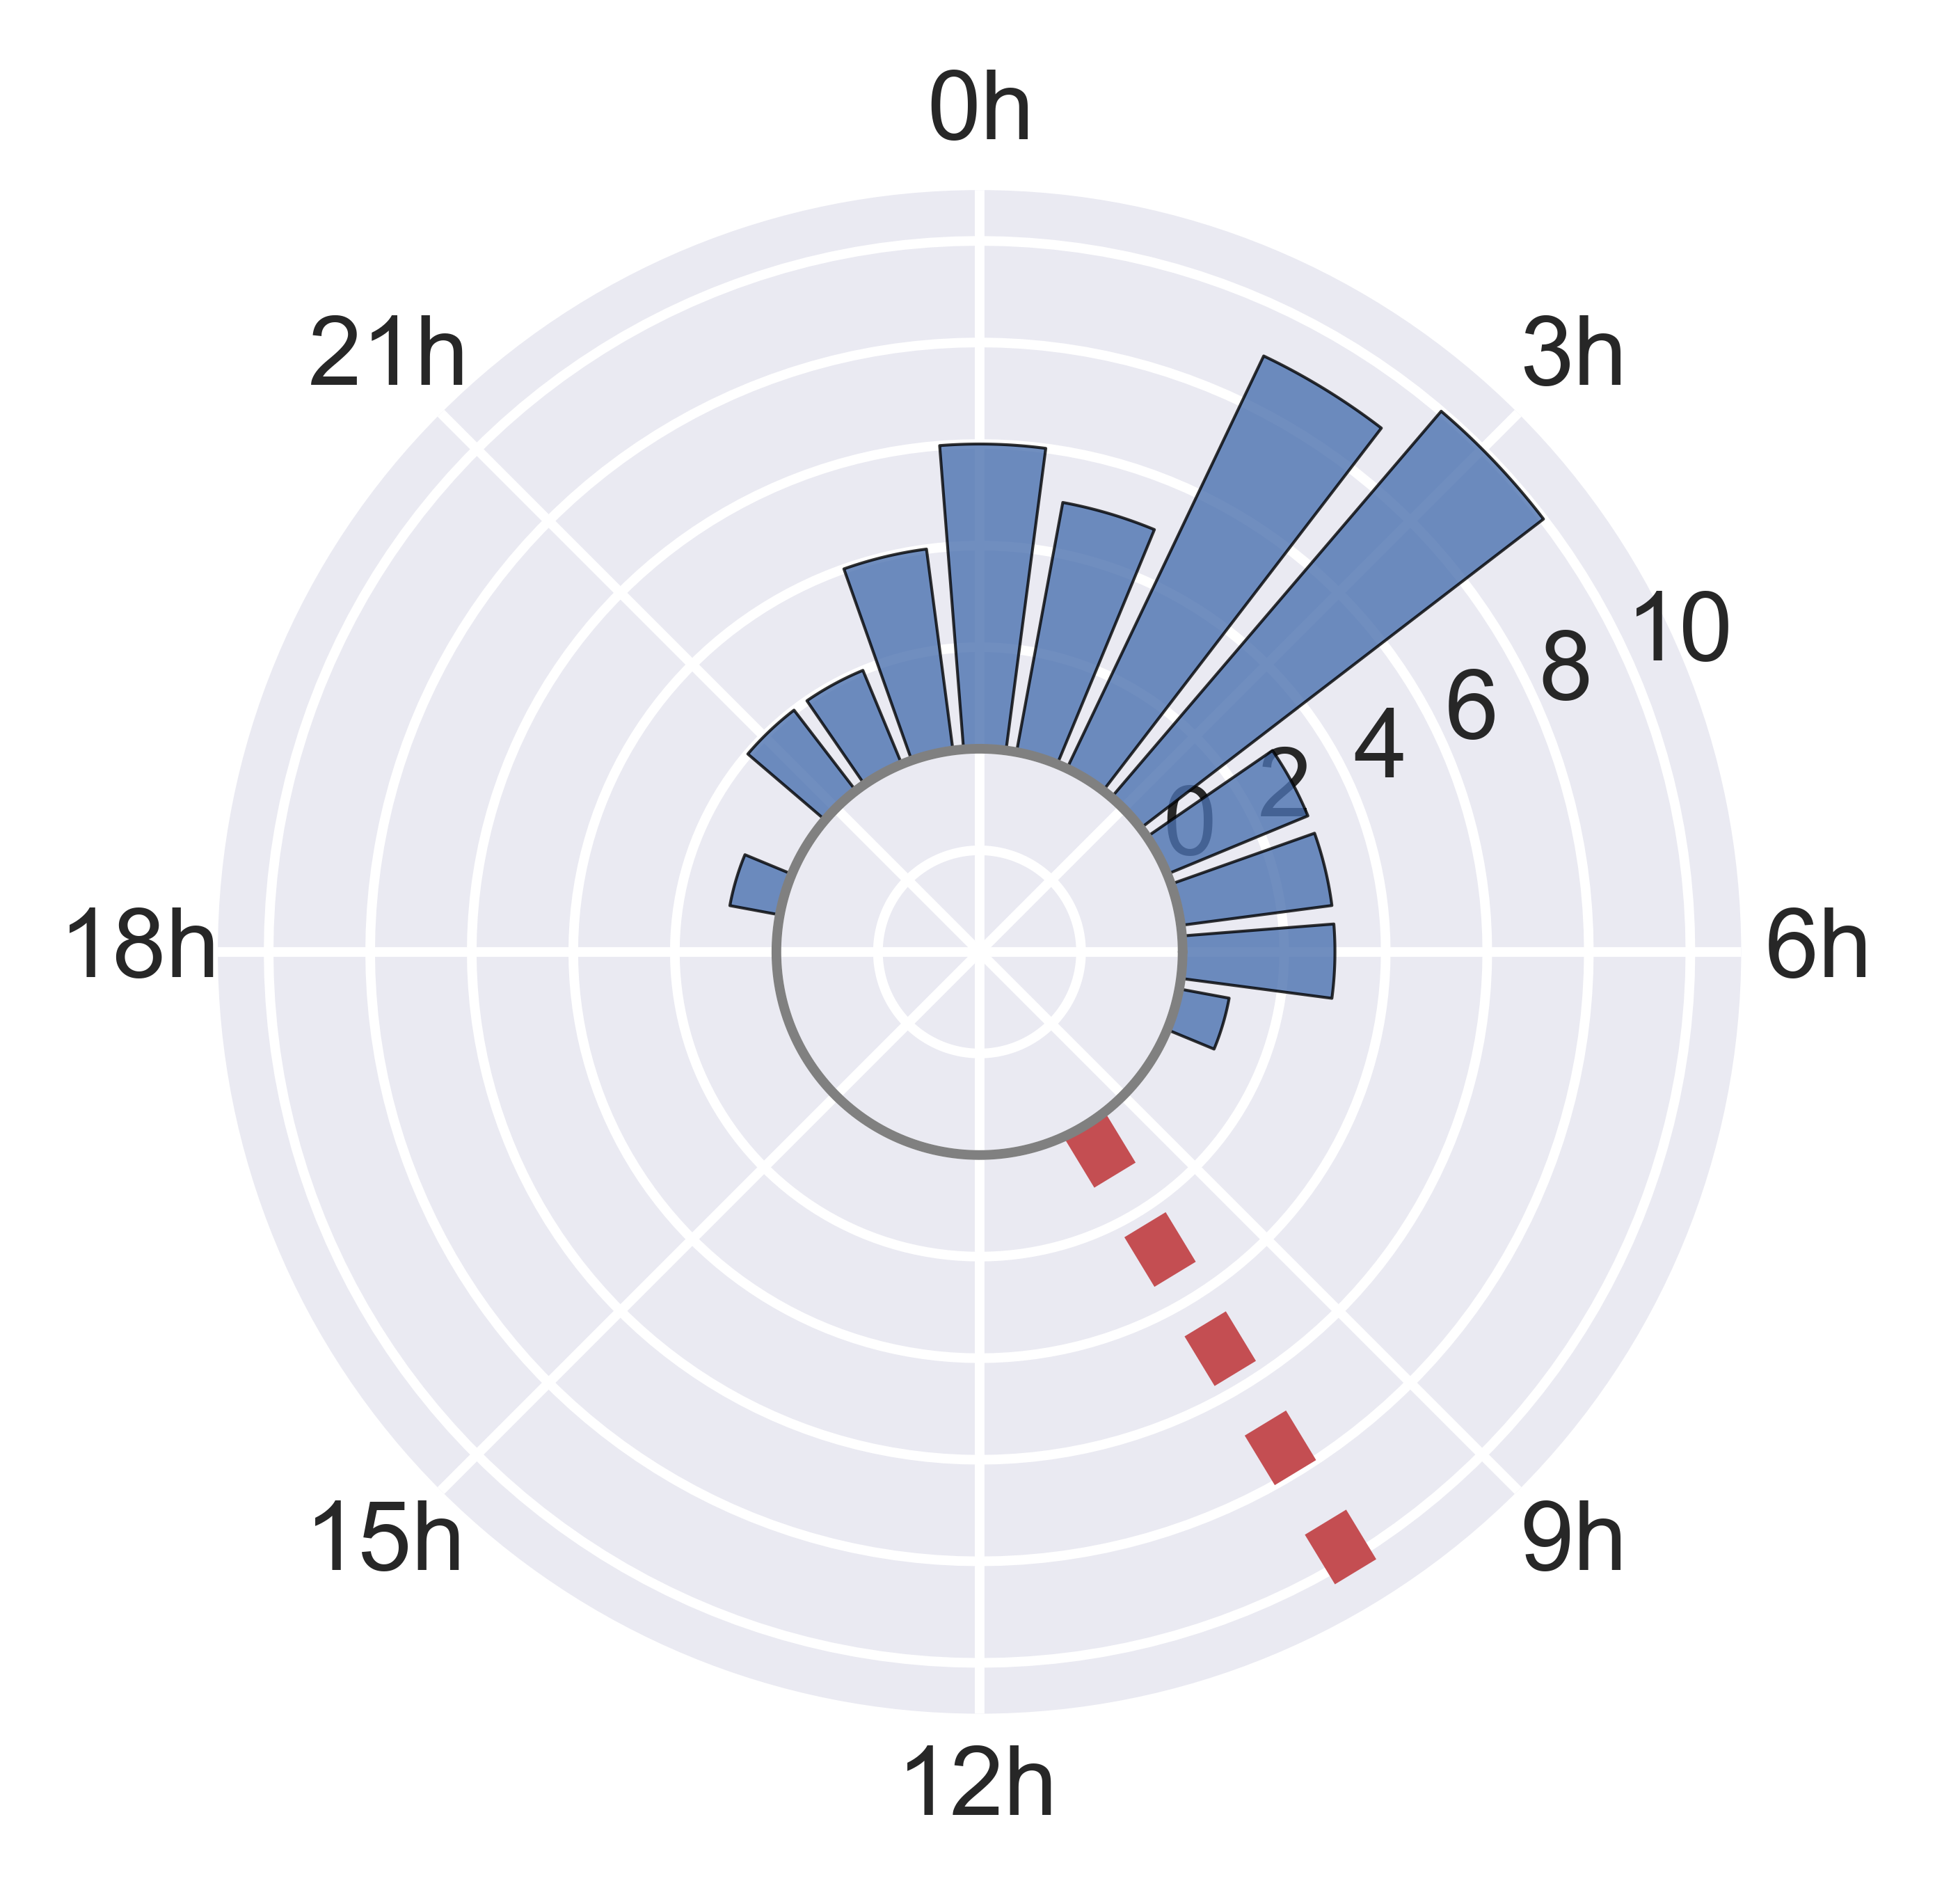
\includegraphics[width=5.5cm]{ch3_fig_1c}\label{fig:von1}}
		\hfill
		\subfloat[Fitted von Mises 
distribution]{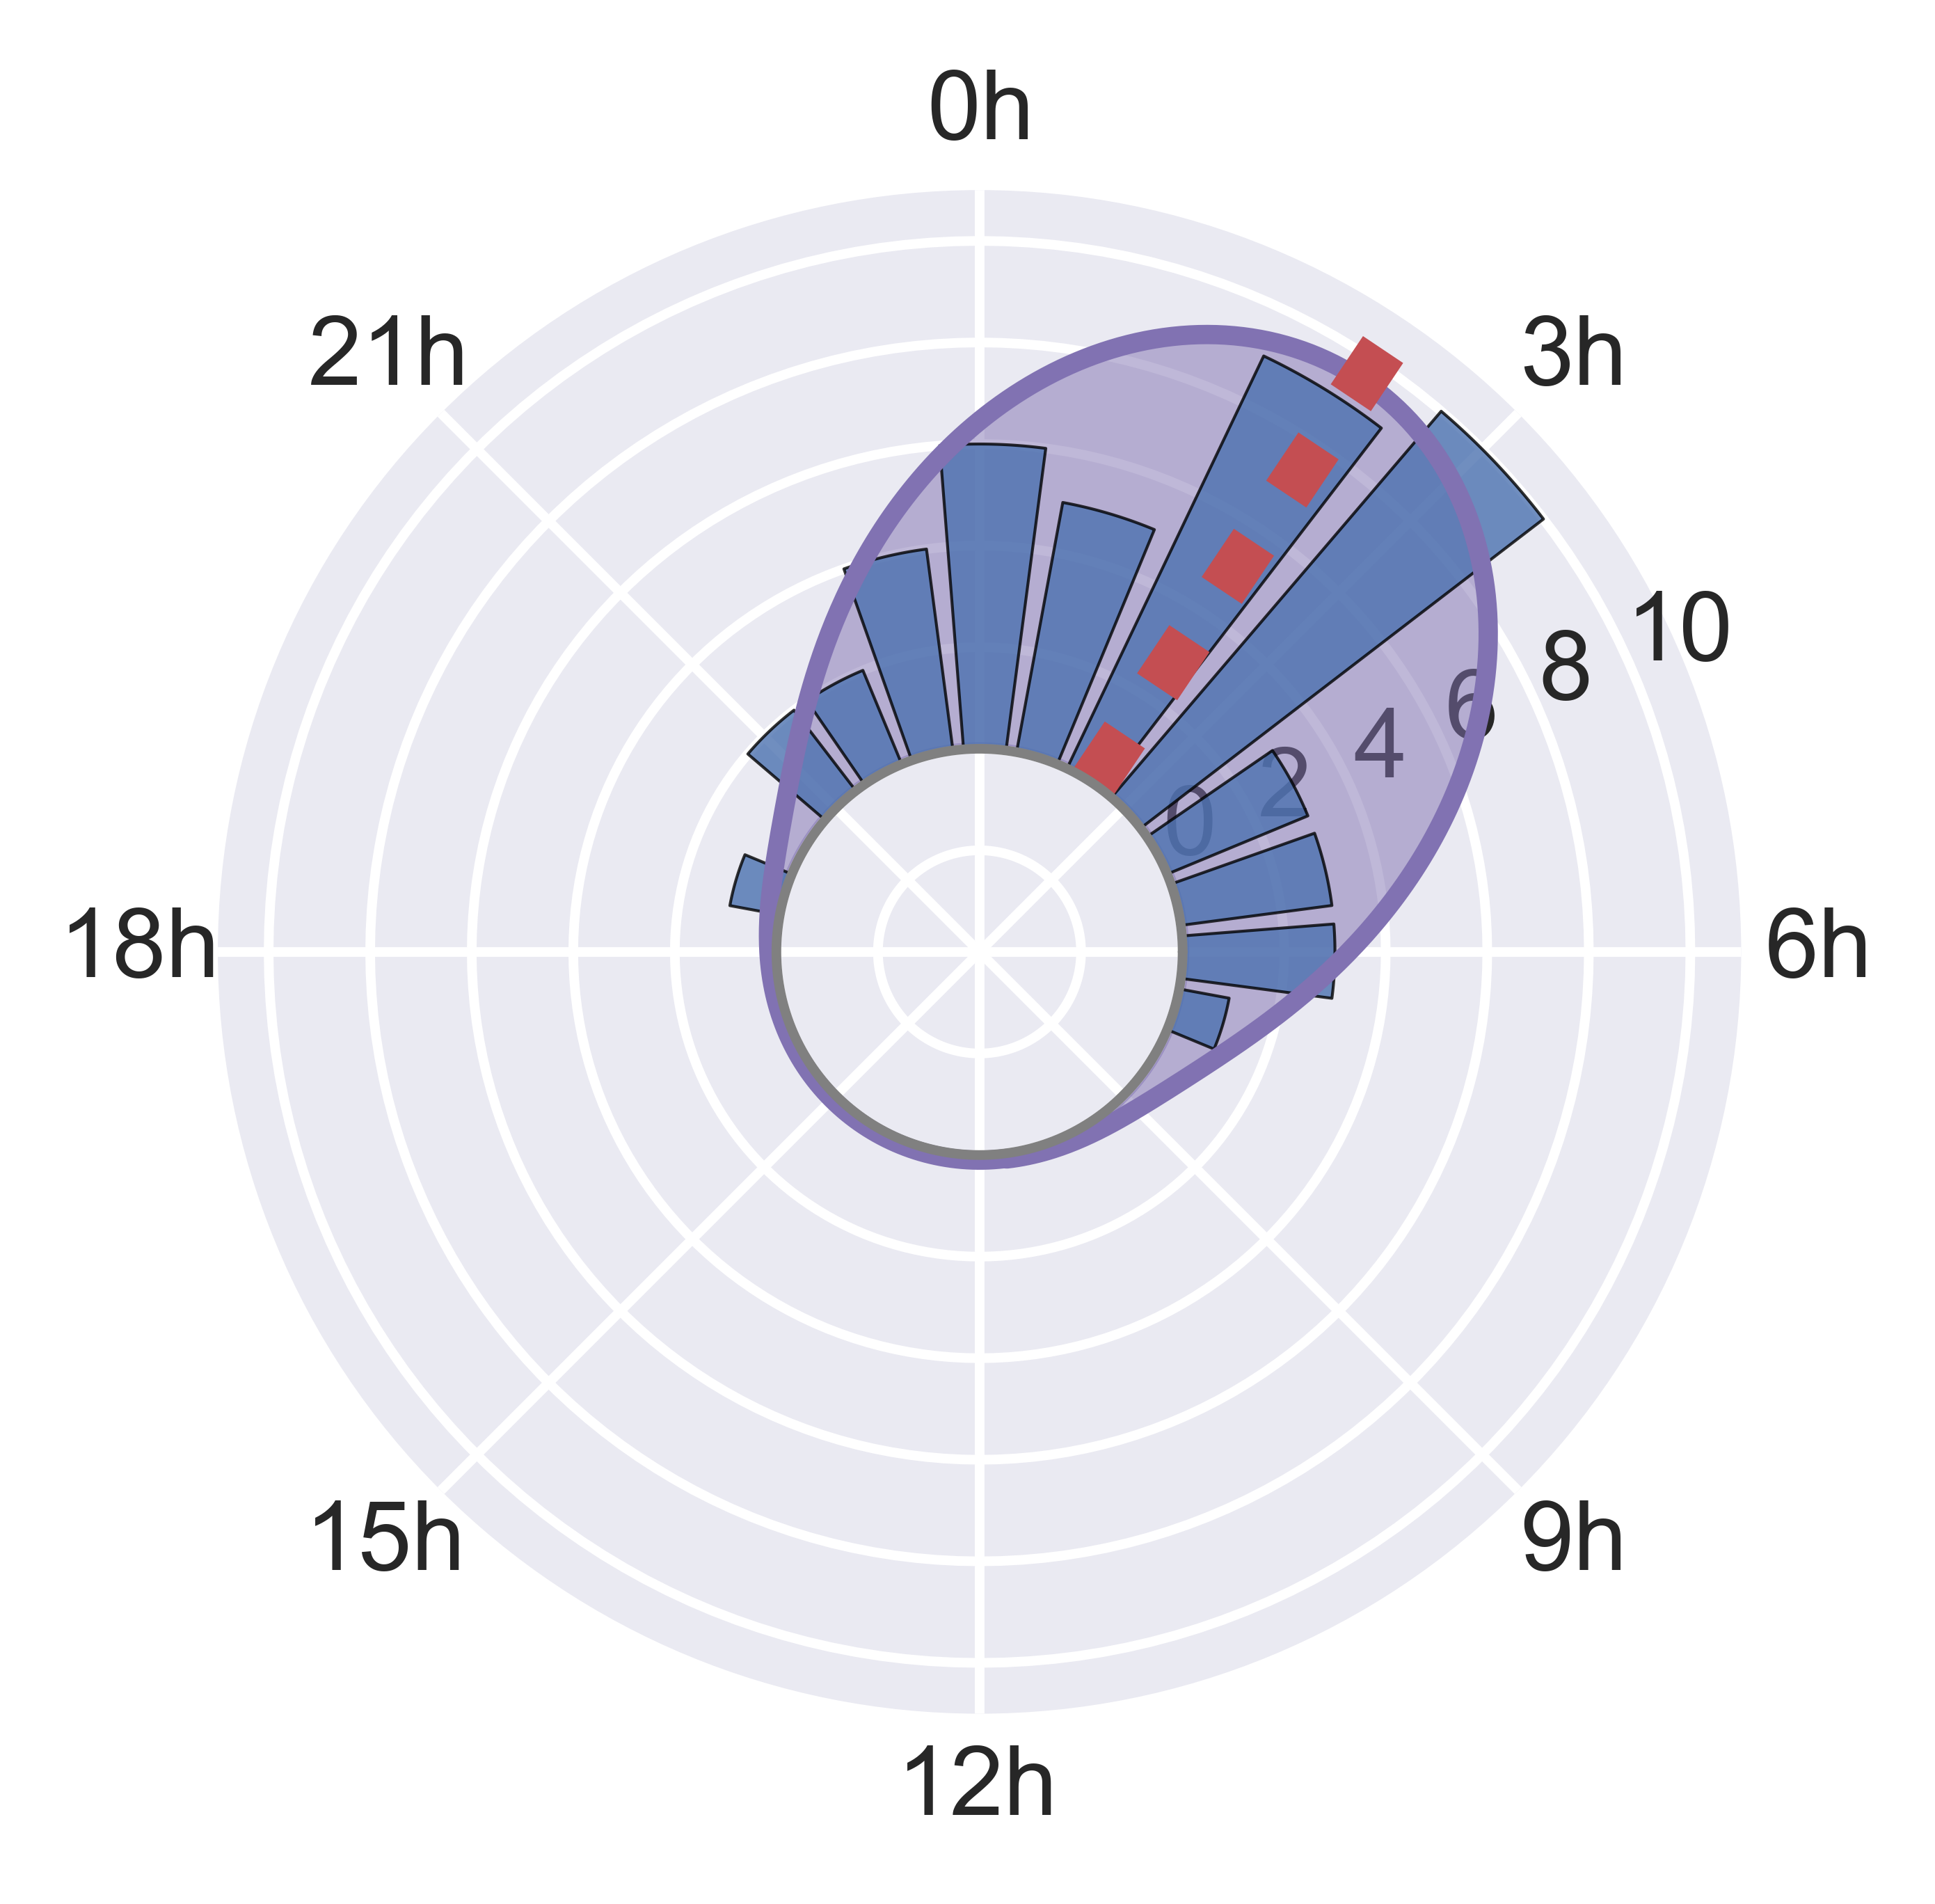
\includegraphics[width=5.5cm]{ch3_fig_2c}\label{fig:von2}}
		\\
		\subfloat[Expected time of 
transaction]{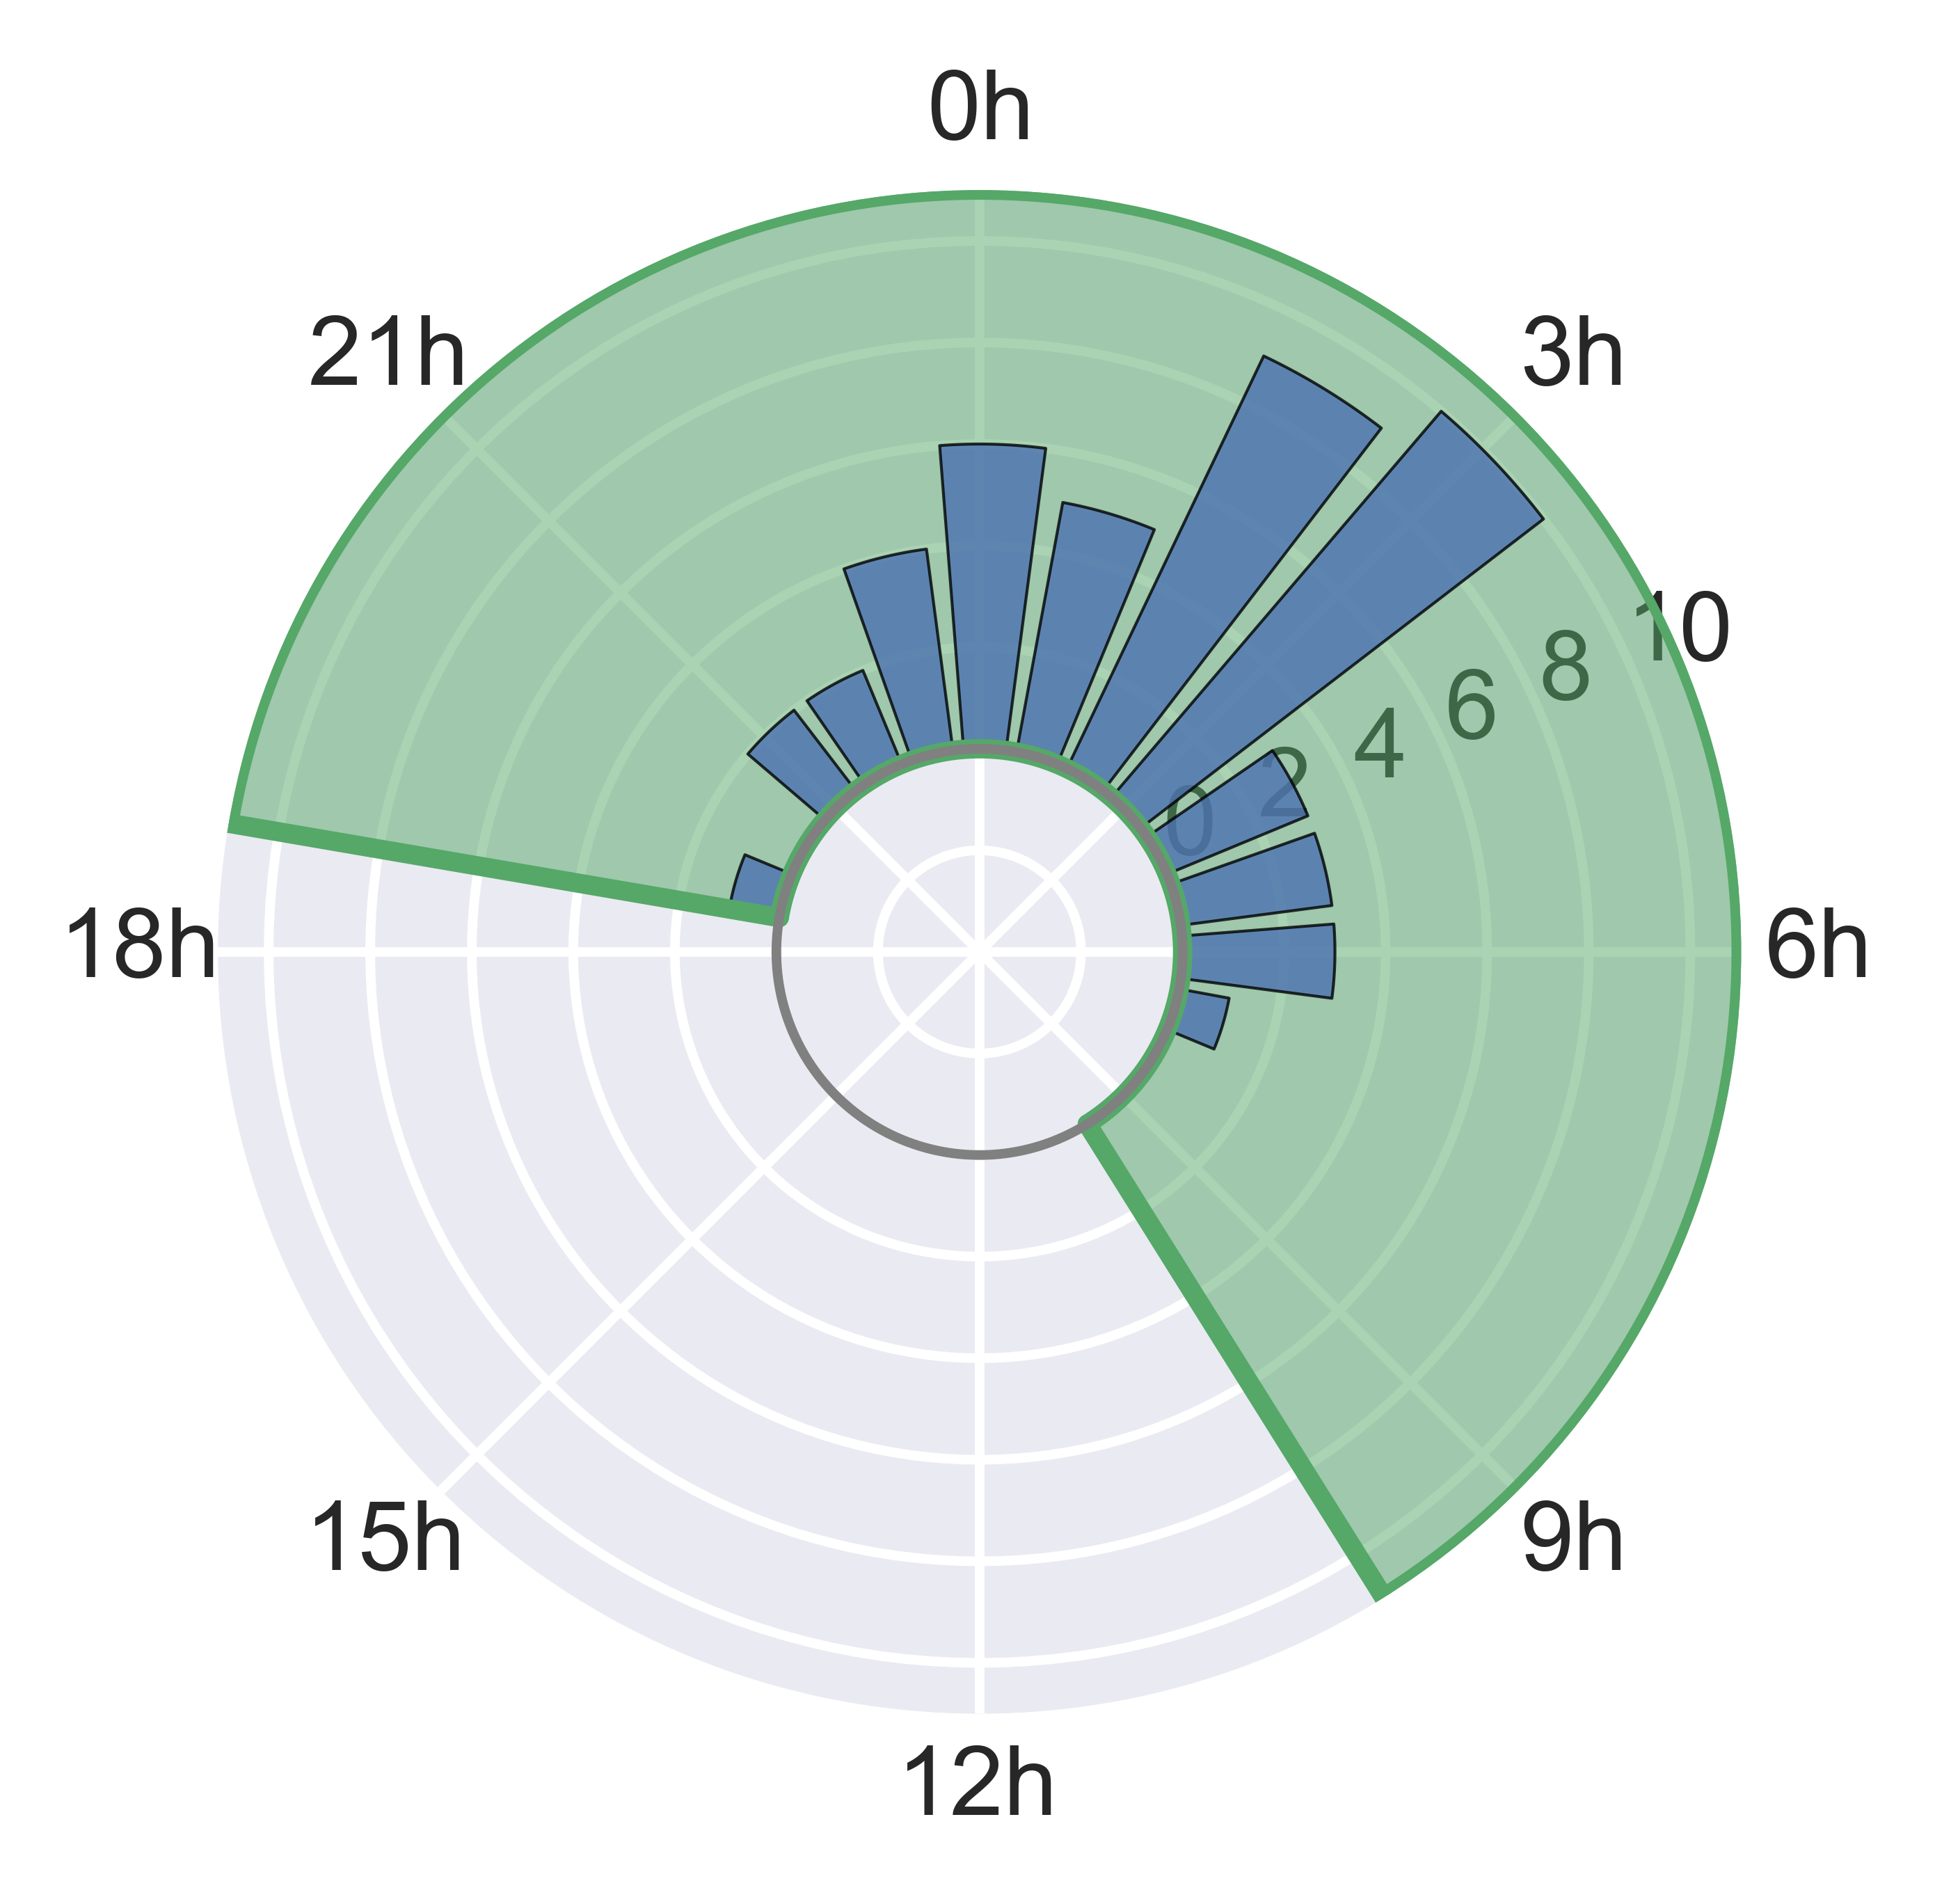
\includegraphics[width=5.5cm]{ch3_fig_3c}\label{fig:von3}}
		\caption{\textbf{Analysis of the time of a transaction using a 24 hour clock and the von Mises 
		distribution.} It is shown that the arithmetic mean of the time of a set of a transaction (a) 
		and the 	periodic mean (b), are completely 	different. Because, the arithmetic mean does not 
		take 		into 	account the periodic behavior of the 	time feature. Moreover, 	by modeling the 
		time of the 		transaction using the von Mises 	distribution (b), a confidence 	interval (c) 
		is estimated. Using 		the confidence interval, a 	transaction can be flag as normal 	or	 
		suspicious, depending 		whether or 	not the time of the 	transaction is within the 	
		confidence 	interval.}
		\label{fig_sim2}
  \end{figure} 
	
	In \figurename{ \ref{fig:von2}}, the von Mises distribution calculation is shown.
	Lastly, using the estimated distribution a new set of features can be develop, ie. a binary 	
	feature ($x_i^{p1}$) if a new transaction time is within the confidence interval range with 
	probability 	$\alpha$.	An example is presented in \figurename{ \ref{fig:von3}}. 
	Furthermore, other features can be calculated, as the confidence interval range can be calculated 
	for several values of $\alpha$, and also the time period can have an arbitrary size.

	\begin{table}[!t]
   \caption{Example calculation of periodic features.}
   \label{tab:agg_features_example2}
   \centering
   \begin{tabular}{|c c | c c c c|}
   \hline
   \multicolumn{2}{|c|}{\textbf{Raw features}} & \multicolumn{4}{c|}{\textbf{Periodic features}} 
		\\  \hline
   \textbf{Id} & \textbf{Time} & \textbf{Arithmetic mean} & \textbf{Periodic mean} & 
		\textbf{Periodic CI} & $x_i^{p1}$ \\
   \hline
		1& 01/01/15 18:20& --- & ---	 &	--- & ---\\
		2& 01/01/15 20:35& --- & ---	 &---	 & ---\\
		3& 01/01/15 22:30& 19:27 & 19:27 & 15:45 - 23:10 & True \\
		4& 02/01/15 00:50& 20:28 & 20:28 & 17:54 - 23:03 & False\\
		5& 02/01/15 19:18& 16:34 & 22:34 & 18:51 - 00:17 & True\\
		6& 02/01/15 23:45& 16:19 & 21:07 & 15:21 - 02:52 & True\\
		7& 03/01/15 06:00& 18:33 & 22:33 & 17:19 - 01:46 & False\\
   \hline
   \end{tabular}
   \end{table}

	Additionally, using the same example as we show used to calculate the aggregated features, 
	we calculate a feature $x_i^{p1}$, as a binary feature that takes the value of one if the current 
	time of the transaction is within the confidence interval of the time of the previous 
	transactions with a confidence of $\alpha=0.9$. The example is show in \tablename{ 
	\ref{tab:agg_features_example2}}. In this example, it is shown, how the arithmetic and periodic 
	means differ, as for the last transaction both means are significantly different. Moreover, the 
	new feature, help to get a felling of when a customer is expected to make transactions.
	
	Finally, when calculating the periodic features, is important to use longer time frames $t_p$, 
	since if the distribution is calculated using only a couple of transactions it may not be as 
	relevant of a customer behavior patterns, compared against using a full year of transactions.
	Evidently, if $t_c$ is less than 24 hours, any transaction made afterwards will not be expected 
	to be within the distribution of previous transactions times. To avoid this we recomend using at 
	least the previous 7 days of transactional information.
	Lastly, this approach can also be used to estimate features such as the expected day of the week 
	of transactions, as some customers may only use their credit cards during the weekend nights, or 
	during working hours.
	
	\subsection{Database}

 	For this paper we used a dataset provided by a large European card processing company. The 
	dataset consists of fraudulent and legitimate transactions made with credit and debit cards 
	between January 2012 and June 2013. The total dataset contains 120,000,000 individual 
	transactions, each one with 27 attributes, including a fraud label indicating whenever a 
	transaction is identified as fraud. This label was created internally in the card processing 
	company, and can be regarded as highly accurate. In the dataset only 40,000 transactions were 
	labeled as fraud, leading to a fraud ratio of 0.025\%. 

	Furthermore, using the methodologies for feature extraction described in Section 
	\ref{sec:features}, we estimate a total of 293 features. Also,
	for the experiments, a smaller subset of transactions with a higher fraud ratio, corresponding 
	to a specific group of transactions, is selected. This dataset contains 236,735 transactions 
	and a fraud ratio of 1.50\%. In this dataset, the total financial losses due to fraud are 
	895,154 Euros. This dataset was selected because it is the one where most frauds are being 
	made. Then, 3 different datasets are extracted: train, validation and test. Each one containing 
	50\%, 25\% and 25\% of the transactions respectively. Afterwards an under-sampling of the 
	legitimate transactions is made, in order to have a balanced class distribution. 
	Additionally, we perform the cost-proportionate rejection-sampling and cost-proportionate 
	over-sampling procedures presented in Section \ref{sec:cs}.	\mbox{\tablename{ 
	\ref{tab:datasets}}}, summarizes the different datasets.  It is important to note that the 
	sampling procedures were only applied to the training dataset since the validation and test 
	datasets must reflect the real fraud distribution.
	
	\begin{table}[t]
	\caption{Summary of the datasets}
	\label{tab:datasets}
	\centering
	\begin{tabular}{l c c c } %sum 7.7
		\\
		\hline
		\textbf{Set}&	\textbf{Transactions} &	\textbf{\%Frauds} & 
		\textbf{Cost} \\
		\hline
		Total&236,735&1.50&895,154\\
		Training&94,599&1.51&358,078\\
		Under-sampled&2,828&50.42&358,078\\
		CS-Rejection-sampled&94,522&1.43&357,927\\
		CS-Over-sampled&189,115&1.46&716,006\\
		Validation&70,910&1.53&274,910\\
		Testing&71,226&1.45&262,167\\
		\hline
	\end{tabular}
\end{table}


\section{Credit scoring}

  In order to mitigate the impact of credit risk and make more objective and accurate decisions, 
  financial institutions use credit scores to predict and control their losses.
  The objective in credit scoring is to classify which potential customers are likely to default a 
  contracted financial obligation based on the customer's past financial experience, and with that 
  information decide whether to approve or decline a loan~\citep{Anderson2007}. This tool has 
  become a standard practice among financial institutions around the world in order to predict 
  and control their loans portfolios. When constructing credit scores, it is a common practice to 
  use standard cost-insensitive binary classification algorithms such as logistic regression, 
  neural networks, discriminant analysis, genetic programing, decision trees, among 
  others~\citep{Hand1997,Bahnsen2011}. 
  
  Formally, a credit score is a statistical model that allows the estimation of the probability 
  $\hat p_i=P(y_i=1|X_i)$ of a customer $i$ defaulting a contracted debt. Additionally, since the 
  objective of credit scoring is to estimate a classifier $c_i$ to decide whether or not to grant a 
  loan to a customer $i$, a threshold $t$ is defined such that if $\hat p_i <t$, then the loan is 
  granted, i.e., $c_i(t)=0$, and denied otherwise, i.e., $c_i(t)=1$.
  
  There exists different approaches for defining the probability threshold. The sensitivity versus 
  specificity ($SvsS$) approach is the most widely used among financial institutions 
  \citep{Anderson2007}, where specificity is the true positive rate $F_0(t)$ for a threshold $t$, 
  and the sensitivity is one minus the false positive rate $F_1(t)$ given a threshold $t$ 
  \citep{Hernandez-Orallo2012}. In this method the objective is to fix the threshold at the point 
  where the sensitivity is equal to the specificity $F_0(t)=1-F_1(t)$, where $F_0(t)$ and $F_1(t)$ 
  are calculated using:
  \begin{equation}
   F_k(t)=\frac{1}{n_k}\vert \{ ( x_i,y_i ) \in D_k \vert \hat p_i \le t \}\vert, \text{ for } 
   k\in\{0,1\}.
  \end{equation}
  Lastly, the $SvsS$ threshold $t_{SvsS}$ is found by using
  \begin{equation}
  t_{SvsS}= \argmin_t \vert F_0(t) - (1-F_1(t)) \vert.
  \end{equation}
  This process is further clarify in \figurename{ \ref{fig:ch3:4}}.
  
  \begin{figure}
  \centering
  \centering
  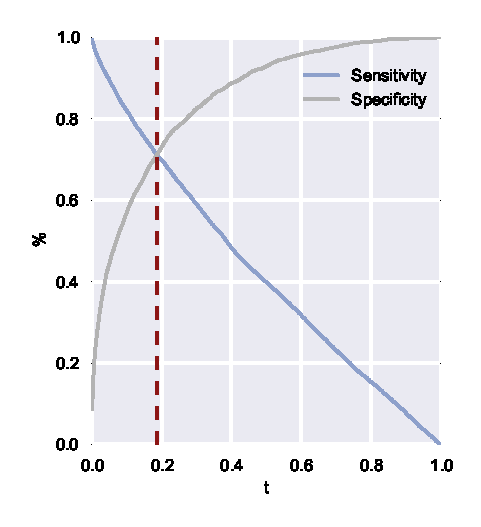
\includegraphics{ch3_fig_4}
  \caption{Credit scoring sensitivity versus specificity thresholding procedure.}
  \label{fig:ch3:4}
  \end{figure}
  
  After the classifier $c_i$ is estimated, there is a need to evaluate its performance. In 
  practice, many statistical evaluation measures are used to assess theperformance of a credit 
  scoring model. Measures such as the area under the  receiver operating characteristic curve (AUC),
  Brier score, Kolmogorov-Smirnoff (K-S) statistic,  $F_1$-Score, and misclassification are among 
  the most common \citep{Beling2005}. Nevertheless, none of these measures takes into account the 
  business and economical realities that take place in credit scoring. Costs that the financial 
  institution had incurred to acquire customers, or the expected profit due to a particular client, 
  are not considered in the evaluation of the different models. This is explored in detail in the 
  next section.

  
  \subsection{Financial evaluation of a credit scorecard }
  
  Typically, a credit risk model is evaluated using standard cost-insensitive measures.
  However, in practice, the cost associated with approving 
  what is known as a bad customer, i.e., a customer who default his credit loan, is quite 
  different from the cost associated with declining a good customer,  i.e., a customer who 
  successfully repay his credit loan. Furthermore, the costs are not constant among customers. 
  This is because loans have different credit line amounts, terms, and even interest rates. Some 
  authors have proposed methods that include the misclassification costs in the credit scoring 
  context \citep{Verbraken2014,Alejo2013,Beling2005,Oliver2009}. However, they assume a constant 
  misclassification cost, which is not the case in credit scoring.
  
 
  Initial approaches to include the different costs have been published in recent years, 
  particularly the one proposed by Beling et al. \citep{Beling2005,Oliver2009}, in which the costs 
  of misclassification are assigned for each error. Specifically, setting the cost of a false 
  positive $C_{FP}$ to the loan's annual interest rate charged to the customer $int_r$, the cost of 
  a false negative $C_{FN}$ to the loss given default $L_{gd}$, which is the percentage of loss 
  over the total credit line when the customer defaulted, and setting to zero the costs of true 
  positive $C_{TP}$ and true negative $C_{TN}$. Using that, they proposed the expected cost (EC) 
  method to find the probability threshold that minimizes those costs, $t_{ec}= 
  \frac{C_{FN}}{C_{FN}+C_{FP}} =\frac{L_{gd}}{L_{gd}+int_r}.$ Nevertheless, this approach assumes 
  a constant cost within examples, which is a strong assumption, since in practice each example 
  carries a very different cost, given by the different credit limits and conditions of each loan. 
  Consequently, there is a need for an example-dependent cost matrix that takes into account the 
  cost of misclassifying each example.
   
  In order to take into account the varying costs that each example carries, we proposed in 
  \citep{CorreaBahnsen2014b}, a cost matrix with example-dependent misclassification costs as 
  given in \tablename{ \ref{table_costmat2}}. First, we assume that the costs of a correct 
  classification, $C_{TP_i}$ and $C_{TN_i}$, are zero for every customer $i$. We define $C_{FN_i}$ 
  to be the losses if the customer $i$ defaults to be proportional to his credit line $Cl_i$. We 
  define the cost of a false positive per customer $C_{FP_i}$ as the sum of two real financial 
  costs $r_i$ and $C^a_{FP}$, where $r_i$ is the loss in profit by rejecting what would have been a 
  good customer. 
  
  \begin{table}
  \caption{Credit scoring example-dependent cost matrix}\label{table_costmat2}
    \centering
    \begin{tabular}{c|c|c}
    %\cline{2-3}
      \multicolumn{1}{c|}{}  & Actual Positive& Actual Negative \\
      \multicolumn{1}{c|}{} & $y_i=1$& $y_i=0$ \\
      \hline
      Predicted Positive& \multirow{ 2}{*}{$C_{TP_i}=0$} & \multirow{2}{*}{$C_{FP_i}=r_i+C^a_{FP}$} 
      \\
      $c_i=1$ & &\\
      \hline
      Predicted Negative& \multirow{ 2}{*}{$C_{FN_i}=Cl_i \cdot L_{gd}$} & \multirow{
      2}{*}{$C_{TN_i}=0$} \\
      $c_i=0$ & &\\
    \end{tabular}
  \end{table}
  
  The profit per customer $r_i$ is calculated as the present value of the difference between the 
  financial institution gains and expenses, given the credit line $Cl_i$, the term $l_i$ and the 
  financial institution lending rate $int_{r_i}$ for customer $i$, and the financial institution 
  of cost funds $int_{cf}$.
  \begin{equation}
    r_i= PV(A(Cl_i,int_{r_i},l_i),int_{cf},l_i)-Cl_i,
  \end{equation}
  with $A$ being the customer monthly payment and $PV$ the present value of the monthly payments,
  which are calculated using the time value of money equations \citep{Lawrence2012},
  \begin{eqnarray}
    A(Cl_i,int_{r_i},l_i) &=&  Cl_i \frac{int_{r_i}(1+int_{r_i})^{l_i}}{(1+int_{r_i})^{l_i}-1}, \\
    PV(A,int_{cf},l_i) &=& \frac{A}{int_{cf}} \left(1-\frac{1}{(1+int_{cf})^{l_i}} \right).
  \end{eqnarray}
    
  The second term $C^a_{FP}$, is related to the assumption that the financial institution will not 
  keep the money of the declined customer idle. It will instead give a loan to an alternative 
  customer \citep{Nayak1997}. Since no further information is known about the alternative customer, 
  it is assumed to have an average credit line $\overline{Cl}$ and an average profit $\overline{r}$.
  Given that, 
  \begin{equation}
    C^a_{FP}=- \overline{r} \cdot \pi_0+\overline{Cl}\cdot L_{gd} \cdot \pi_1,
  \end{equation}
  in other words minus the profit of an average alternative customer plus the expected loss, 
  taking into account that the alternative customer will pay his debt with a probability equal to 
  the prior negative rate, and similarly will default with probability equal to the prior positive 
  rate.

  \subsubsection{Calculation of the credit limit}
  
  One key parameter of our model is the credit limit. There exists several strategies to calculate 
  the $Cl_i$ depending on the type of loans, the state of the economy, the current portfolio, 
  among others \citep{Anderson2007,Lawrence2012}. Nevertheless, given the lack of information 
  regarding the specific business environments of the considered datasets, we simply define 
  $Cl_i$ as
  \begin{equation}\label{eq:cli}
      Cl_i = \min \bigg\{ k \cdot Inc_i, Cl_{max}, Cl_{max}(debt_i) \bigg\},
  \end{equation}
  where $Inc_i$ and $debt_i$ are the monthly income and debt ratio of the customer $i$, 
  respectively, $k$ is a parameter that defines the maximum $Cl_i$ in times $Inc_i$, and 
  $Cl_{max}$ the maximum overall credit line. Lastly, the maximum credit line given the current 
  debt is calculated as the maximum credit limit such that the current debt ratio plus the new 
  monthly payment does not surpass the customer monthly income. It is calculated as
  \begin{equation}
    Cl_{max}(debt_i)=PV\left(Inc_i \cdot P_{m}(debt_i),int_{r_i},l_i\right),
  \end{equation}
  and
  \begin{equation}
    P_{m}(debt_i)=\min \left\{ \frac{A(k \cdot Inc_i,int_{r_i},l_i)}{Inc_i},\left(1-debt_i 
    \right) \right\}.
  \end{equation}
  
  
  \subsection{Databases}

    For this paper we use two different publicly available credit scoring datasets. The first 
    dataset is the \textbf{2011 Kaggle competition Give Me Some Credit}\footnote{ 
    http://www.kaggle.com/c/GiveMeSomeCredit/}, in which the objective is to identify those 
    customers of personal loans that will experience financial distress in the next two years.
    The second dataset is from the \textbf{2009 Pacific-Asia Knowledge Discovery and Data Mining 
    conference (PAKDD) competition}\footnote{http://sede.neurotech.com.br:443/PAKDD2009/}.
    Similarly, this competition had the objective of identifying which credit card applicants
    were likely to default and by doing so deciding whether or not to approve their applications.
    The Kaggle Credit and PAKDD Credit datasets contain information regarding the features, and 
    more importantly about the income of each example, from which an estimated credit limit 
    $Cl_i$ can be calculated (see Appendix~\ref{app_cli}).
    
    The Kaggle Credit dataset contains 112,915 examples, each one with 10 features and the class 
    label. The proportion of default or positive examples is 6.74\%. 
    On the other hand, the PAKDD Credit dataset contains 38,969 examples, with 30 features and the 
    class label, with a proportion of 19.88\% positives. This database comes from a Brazilian 
    financial institution, and as it can be inferred from the competition description, the data 
    was obtained around 2004.
    
    Since no specific information regarding the datasets is provided, we assume that they belong to 
    average European and Brazilian financial institutions. This enabled us to find the different 
    parameters needed to calculate the cost measure described in 
    Section~\ref{section_cost_matrices}. In Table~\ref{table_parameters}, the different 
    parameters are shown. In particular, we obtain the average interest rates in Europe during 
    2013 from the European Central Bank \citep{ECB2014}, and the average interest and exchange 
    rates in Brazil during 2004 from Trading Economics \citep{Economics2014}. Because the income 
    is not in the same currency on both datasets, we convert the PAKDD Credit dataset to Euros.
    Additionally, we use a fixed loan term $l$ for both datasets, considering that in the Kaggle 
    Credit dataset the class was constructed to predict two years of credit behavior, and 
    because the PAKDD Credit dataset is related to credit cards the term is fix to two years 
    \citep{Lawrence2012}. Moreover, we set the loss given default $L_{gd}$ using information from 
    the Basel II standard\footnote{http://www.bis.org/publ/bcbsca.htm.}, $k$ to 3 since it is the 
    average personal loan requests related to monthly income, and the maximum credit limit 
    $Cl_{max}$ to 25,000 Euros.
    \todo{table databases}